\documentclass[12pt, a4, english]{article}

\usepackage[T1]{fontenc}
\usepackage[latin1]{inputenc}
\usepackage[nenglish]{babel}	 %use german spellings

\usepackage{../mmm}

\usepackage{color}
\definecolor{grau}{rgb}{0.4,0.4,0.4} 
\definecolor{schwarz}{rgb}{0,0,0} 
\definecolor{BLUE}{rgb}{0.,0.,1.}
\definecolor{RED}{rgb} {1.,0.,0.}
\definecolor{GREEN}{rgb} {0.,.7,0.}

\def\xcolorcmd{\colorlet{black}{gray!150}}
\usepackage{xcolor}

\usepackage{url}
\usepackage{graphicx}
\graphicspath{pics}

\setlength{\parindent}{0em}
\setlength{\textwidth}{17cm}

\newcommand{\red}[1]{\textcolor{RED}{#1}}
\newcommand{\blue}[1]{\textcolor{BLUE}{#1}}
\newcommand{\green}[1]{\textcolor{GREEN}{#1}}

\newcounter{problem}
\newcounter{pointsa}
\newcounter{pointsb}
\newcounter{blatt}

\setcounter{blatt}{1}

\newenvironment{problem}[3]{
  \addtocounter{problem}{1}
  \addtocounter{pointsa}{#1}
  \addtocounter{pointsb}{#2}
  \bigskip 
  {    \textbf{Task \theproblem}: #3 \hrulefill 
%\textsc{Inf}: (\rule{6mm}{0pt} / \textbf{}) - \textsc{Kom}: (\rule{6mm}{0pt} 
 \textbf{}
  }\begin{quote}
  }{  
  \end{quote}}

%http://www.math.tu-dresden.de/~rudl/latex/fonts.pdf

\headheight0.0cm
\topmargin-2.5cm
\oddsidemargin0.0cm
\textwidth15.92cm
\textheight25cm

\usepackage{watermark}
\usepackage{tikz}

\newcommand{\changefont}[3]{
\fontfamily{#1} \fontseries{#2} \fontshape{#3} \selectfont}

\begin{document}

\thiswatermark{
%\centering
%\put(320,-160){\begin{tikzpicture}%
 %           \node (0,0) [opacity=0.05]{%
  %           \includegraphics[width=4.5cm]{../unilogo.png}};%
   %      \end{tikzpicture}}
\put(120,-145){\begin{tikzpicture}%
            \node (0,0) [opacity=0.5]{%
             \includegraphics[width=4.5cm]{../uni-siegel.png}};%
         \end{tikzpicture}}
\put(355,-145){\begin{tikzpicture}%
            \node (0,0) [opacity=0.5]{%
             \includegraphics[width=2.9cm]{../unilogo.pdf}};%
         \end{tikzpicture}}
%\put(115,-145){\includegraphics[width=5cm]{../uni-siegel.png}}
}

\begin{center}
\begin{tabular}[t]{rcl}
\begin{minipage}{3cm}
\vspace*{0.1cm}
\hspace*{-1.8cm}

\includegraphics[width=4.5cm]{../hcm-logo.pdf}
\end{minipage}
&
\begin{minipage}{10cm}
\vspace*{0.5cm}
%\usefont{T1}{phv}{c}{n}\selectfont
\usefont{T1}{phv}{m}{n}\selectfont
{%\normalsize{Universit�t Augsburg}\\
\textcolor{schwarz}{
\normalsize{Institut f�r Informatik\\
Lehrstuhl Human Centered Multimedia\\
\\
\textbf{Prof. Dr. Elisabeth Andr\'e}\\
Simon Flutura
}
}
}
\end{minipage}
\end{tabular}\\
\end{center}
\vspace*{-0.5cm}
\textcolor{schwarz}{\rule{\textwidth}{0.3pt}}
\begin{center}
\usefont{T1}{phv}{b}{n}\selectfont
%\usefont{T1}{uhv}{b}{n}\selectfont
{\Large {\bf{
\usefont{T1}{phv}{b}{n}\selectfont
\vspace*{0.5cm}
\textcolor{schwarz}{SSI on Android, SS 2015}}}}          
\end{center}
\vspace{0.2cm}
%
%
% =====================================================================
%
\shorthandoff{"} % Use Gaensefuesschen within the text without quoting them
\begin{center}
\usefont{T1}{phv}{b}{n}\selectfont{\large
%\usefont{T1}{uhv}{b}{n}\selectfont{\large
\theblatt. Introduction}
\end{center}
\vspace{0.2cm}
%\changefont{ppl}{m}{n}
%\changefont{ptm}{m}{n}
%\changefont{phv}{m}{n}

%\changefont{cmr}{m}{n}

\changefont{phv}{m}{n}
\normalsize

SSI - Social Signal Iterpretation Framework has been portet to Linux with an Android-port in the works.
Devices like the Raspberry PI, as well as several mobile devices can now be used. This guide shows you how to set up SSI on Android\\\\
%------------------------------------------------------------------------------------------------------------------------------------------------------------------------------------------------------------
\begin{problem}{0}{0}{Prepare the setup (\textbf{note:} crosscompile from Windows)}


\begin{enumerate}
\item GCC and G++ 4.8 or later have to be installed, because SSI relies on C++11 standard.
\item CMake is needed as build-system.
\item Android SDK and NDK are needed and has to be setup on the your system.
\item Apache ANT is needed to build an APK and has to be in PATH.
Instructions can be found here:

\verb|https://developer.android.com/ndk/guides/setup.html|
\end{enumerate}
\end{problem}
%------------------------------------------------------------------------------------------------------------------------------------------------------------------------------------------------------------
\begin{problem}{0}{0}{Get SSI}
SSI can be found here:
\begin{enumerate}
	\item from git \verb|https://hcm-lab.de/git/ssi/ssi-pub.git|
\item from subversion \verb|https://hcm-lab.de/svn/Johannes/openssi/trunk/|
\item from \verb|cleanport.tar.gz| archive from:

 \verb|https://skathi.net/pub/simon/ssi/clean_port_.tar.gz|

\end{enumerate}
\end{problem}


\begin{problem}{0}{0}{Prepare Buildsystem for APK}

for apk creation some additional steps are neccessary.
\begin{enumerate}
	\item copy \verb|*| from \verb|trunk/docs/apk| to trunk.
	\item additionally copy  \verb|trunk/docs/apk/android/AndroidManifest.xml| to trunk.
	\item edit android.apk.cmake to match your device regarding \verb|ANDROID_APK_API_LEVEL|
	
\end{enumerate}

	note to rebuild the APK you have to:
	
	\verb|make clean -f plugins\androidSensors\tools\Makefile|

your apk will be build in \verb|trunk/bin_cmake/Apk/bin/|

\end{problem}

%----------------------------------------------------------------------------------------------------------------------------------------------------------------------------------------

\begin{problem}{0}{0}{Build SSI}

Install CMake; create a build directory next to your SSI-root called trunk in the following text.
Start CMake, select trunk as source directory and your build directory..

\textbf{Note} that your binaries will be put to \verb|trunk/bin_cmake| with "make install" the final step.

following variables have to be set to match your device/emulator:

\verb| ANDROID_ABI=armeabi-v7a|

\verb| ANDROID_NATIVE_API_LEVEL=android-21 |

following variables have to be set to match your setup:

\verb| ANDROID_NDK=absolute/path/to/ndk|

\verb| CMAKE_MAKE_PROGRAM=filepath/to/make/binary (NDK/prebuilt/%PLATTFORM%/bin/make.exe)|



Press configure and lets follow the wizard:



\begin{figure}[p]

   \centering
	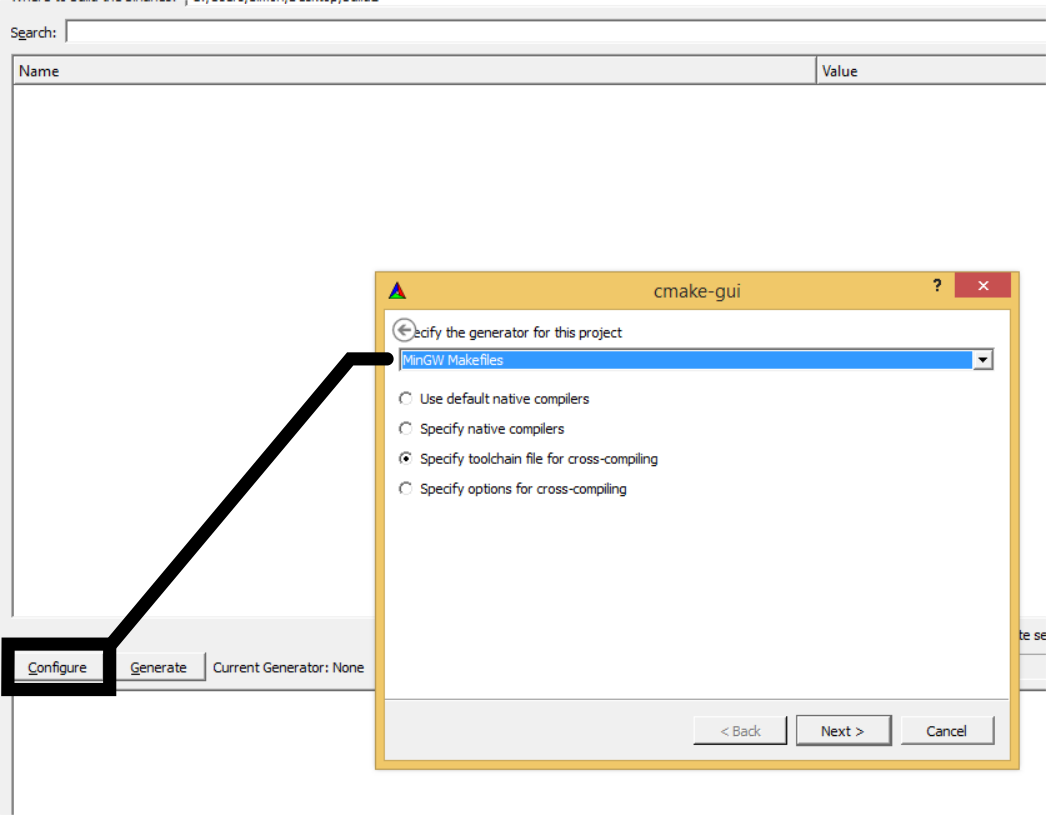
\includegraphics[width=0.8\textwidth]{../screenshots/01.png}
   \caption{In CMake-GUI: select MinGW Makefiles; toolchain for crosscompiling}
   \label{fig:configure_cmake}

\end{figure}



\begin{figure}[p]

   \centering
\includegraphics[width=0.8\textwidth]{../screenshots/02.png}
   \caption{select android.toolchain.cmake from trunk/docs/ssi-port-cmake/intro-android-from-win}
   \label{fig:select_toolchain}

\end{figure}


\begin{figure}[p]

   \centering
\includegraphics[width=0.8\textwidth]{../screenshots/03_.png}
   \caption{Ignore the error}
   \label{fig:error}

\end{figure}

\begin{figure}[p]

   \centering
\includegraphics[width=0.8\textwidth]{../screenshots/04_.png}
   \caption{change to advanced view and add entries fitting your device.   }
   \label{fig:add_entries}

\end{figure}


\begin{figure}[p]

   \centering
\includegraphics[width=0.8\textwidth]{../screenshots/05_.png}
   \caption{marked values should be set; configure; generate}
   \label{fig:overview}

\end{figure}

\begin{figure}[p]

   \centering
\includegraphics[width=0.8\textwidth]{../screenshots/06.png}
   \caption{find your build system in your cmake build dir (where to build the binaries);
   type "make -j6 install" to rebuild the APK first run "make clean"}
   \label{fig:awesome_image}

\end{figure}
\end{enumerate}
\end{problem}



\newpage
%----------------------------------------------------------------------------------------------------------------------------------------------------------------------------------------

\begin{problem}{0}{0}{Prepare Buildsystem for APK}

for apk creation some additional steps are neccessary.
\begin{enumerate}
	\item setup ant build system to be in PATH
	\item copy \verb|*| from \verb|trunk/docs/apk| to trunk.
	\item additionally copy  \verb|trunk/docs/apk/android/AndroidManifest.xml| to trunk.
	\item edit android.apk.cmake to match your device regarding \verb|ANDROID_APK_API_LEVEL|
	
\end{enumerate}

your apk will be build in \verb|trunk/bin_cmake/Apk/bin/|

\end{problem}

%----------------------------------------------------------------------------------------------------------------------------------------------------------------------------------------

\begin{problem}{0}{0}{Run tests}
Your freshly build binarys are located in ssi roots \verb|bin_cmake| directory:

\verb|trunk/cmake_bin/Android|

(keep in mind where your SDK is placed; if it is not in PATH adapt commands below!)

\begin{enumerate}
	\item create and start your emulator:
	
	\verb|android create avd -t 2 -n name|
	
	where -t names the correct target from android list targets	
	
	\item copy files to emulator:
	
	\verb|adb -e push trunk/cmake_bin/Android /data/test|
	
	\verb|adb -e shell chmod 777 /data/test/*|
	
	\verb|adb -e shell|

	\item Set the \verb|LD_LIBRARA_PATH| 
	
	\verb|export LD_LIBRARY_PATH=".:/system/lib/"|
	 or fixed to the SSI root path, so shared libraries can be found.

	\item To test a simple pipeline:
	then run \verb|./ssiandroid_test| from \verb|data/test/|.
	The correct working directory is needed, so the shared plugins can be found.
	
	\item Apart from c++ code one can as well run xml pipelines via:
	
	\verb|./xmlpipe test.pipeline|
	

	\item The same steps are valid for rooted Android devices.
	Use \verb|adb -d| to connect to your device.
	

	

\end{enumerate}
\end{problem}
%----------------------------------------------------------------------------------------------------------------------------------------------------------------------------------------

\begin{problem}{0}{0}{Choose IDE}
To further develop SSI on Linux QtCreator is recommended.
Do not forget to install the GNU debugger GDB.

For better Android Integration Android-Studio might be a wise choise.

Setting up remote GDB follows..

Have fun.

\end{problem}

\end{document}


